%%%%%%%%%%%%%%%%%%%%%%%%%%%%%%%%%%%%%%%%%%%%%%%%%%%%%%%%%%%%%%%%%%%%%%%%%%%%%%%
% Full instructions available at:
% https://github.com/elauksap/focus-beamertheme

\documentclass{beamer}
\usetheme{focus}

% package for font
\usepackage{fontspec}
\defaultfontfeatures{Mapping=tex-text}  %%如果没有它,会有一些 tex 特殊字符无法正常使用,比如连字符。
\usepackage{xunicode,xltxtra}
\usepackage[BoldFont,SlantFont,CJKnumber,CJKchecksingle]{xeCJK}  % \CJKnumber{12345}: 一万二千三百四十五
\usepackage{CJKfntef}  %%实现对汉字加点、下划线等。
\usepackage{pifont}  % \ding{}
% package for math
\usepackage{amsfonts}
% package for graphics
\usepackage[americaninductors,europeanresistors]{circuitikz}
\usepackage{tikz}
\usetikzlibrary{plotmarks}  % placements=positioning
\usepackage{graphicx}  % \includegraphics[]{}
\usepackage{subfigure}  %%图形或表格并排排列
% package for table
\usepackage{colortbl,dcolumn}  %% 彩色表格
\usepackage{multirow}
\usepackage{multicol}
\usepackage{booktabs}
% package for code
\usepackage{fancyvrb}
\usepackage{listings}
% setting for font
%%\setCJKmainfont{Adobe Kaiti Std}
\setCJKmainfont{SimSun}
%%\setCJKmainfont{Microsoft YaHei}
%%\setCJKmainfont{FangSong_GB2312} 
%%\setmainfont{Times New Roman}
%\setsansfont[Mapping=tex-text]{Adobe Song Std}
%如果装了Adobe Acrobat,可在font.conf中配置Adobe字体的路径以使用其中文字体。
%也可直接使用系统中的中文字体如SimSun、SimHei、微软雅黑等。
%原来beamer用的字体是sans family;注意Mapping的大小写,不能写错。
%设置字体时也可以直接用字体名,以下三种方式等同:
%\setromanfont[BoldFont={黑体}]{宋体}
%\setromanfont[BoldFont={SimHei}]{SimSun}
%\setromanfont[BoldFont={"[simhei.ttf]"}]{"[simsun.ttc]"}

% font setting by xeCJK
\setCJKfamilyfont{NSimSun}{NSimSun}
\newcommand{\song}{\CJKfamily{NSimSun}}
%%%\setCJKfamilyfont{AdobeSongStd}{Adobe Song Std}
%%%\newcommand{\AdobeSong}{\CJKfamily{AdobeSongStd}}
\setCJKfamilyfont{FangSong}{FangSong_GB2312}
\newcommand{\fang}{\CJKfamily{FangSong}}
%%%\setCJKfamilyfont{AdobeFangsongStd}{Adobe Fangsong Std}
%%%\newcommand{\AdobeFang}{\CJKfamily{AdobeFangsongStd}}
\setCJKfamilyfont{SimHei}{SimHei}
\newcommand{\hei}{\CJKfamily{SimHei}}
%%%\setCJKfamilyfont{AdobeHeitiStd}{Adobe Heiti Std}
%%%\newcommand{\AdobeHei}{\CJKfamily{AdobeHeitiStd}}
\setCJKfamilyfont{KaiTi}{KaiTi_GB2312}
\newcommand{\kai}{\CJKfamily{KaiTi}}
%%%\setCJKfamilyfont{AdobeKaitiStd}{Adobe Kaiti Std}
\newcommand{\AdobeKai}{\CJKfamily{AdobeKaitiStd}}
\setCJKfamilyfont{LiSu}{LiSu}
\newcommand{\li}{\CJKfamily{LiSu}}
\setCJKfamilyfont{YouYuan}{YouYuan}
\newcommand{\you}{\CJKfamily{YouYuan}}
\setCJKfamilyfont{FZJingLei}{FZJingLeiS-R-GB}
\newcommand{\jinglei}{\CJKfamily{FZJingLei}}
\setCJKfamilyfont{MSYH}{Microsoft YaHei}
\newcommand{\msyh}{\CJKfamily{MSYH}}

\setbeamerfont{frametitle}{series=\Large\hei} % 修改Beamer标题字体

\graphicspath{{figures/}}  %%图片路径
\renewcommand\figurename{图}

% setting for pdf
\hypersetup{% pdfpagemode=FullScreen,%
  pdfauthor={Xiaodong Wang},%
  pdftitle={Title},%
  CJKbookmarks=true,%
  bookmarksnumbered=true,%
  bookmarksopen=false,%
  plainpages=false,%
  colorlinks=true,%
  citecolor=green,%
  filecolor=magenta,%
  linkcolor=blue,%red(default)
  urlcolor=cyan}

% setting for fontspec
\XeTeXlinebreaklocale "zh"  %%表示用中文的断行
\XeTeXlinebreakskip = 0pt plus 1pt minus 0.1pt  %%多一点调整的空间
%%%%%

% 自定义颜色
\def\Red{\color{red}}
\def\Green{\color{green}}
\def\Blue{\color{blue}}
\def\Mage{\color{magenta}}
\def\Cyan{\color{cyan}}
\def\Brown{\color{brown}}
\def\White{\color{white}}
\def\Black{\color{black}}

\lstnewenvironment{xmlCode}[1][]{% for Java
  \lstset{
    basicstyle=\tiny\ttfamily,%
    columns=flexible,%
    framexleftmargin=.7mm, %
    % frame=shadowbox,%
    % rulesepcolor=\color{cyan},%
     frame=single,%
    backgroundcolor=\color{white},%
    xleftmargin=4\fboxsep,%
    xrightmargin=4\fboxsep,%
    numbers=left,numberstyle=\tiny,%
    numberblanklines=false,numbersep=7pt,%
    language=xml, %
    }\lstset{#1}}{}

\lstnewenvironment{javaCode}[1][]{% for Java
  \lstset{
    basicstyle=\tiny\ttfamily,%
    columns=flexible,%
    framexleftmargin=.7mm, %
    frame=shadowbox,%
    rulesepcolor=\color{cyan},%
    % frame=single,%
    backgroundcolor=\color{white},%
    xleftmargin=4\fboxsep,%
    xrightmargin=4\fboxsep,%
    numbers=left,numberstyle=\tiny,%
    numberblanklines=false,numbersep=7pt,%
    language=Java, %
    }\lstset{#1}}{}

\lstnewenvironment{shCode}[1][]{% for Java
  \lstset{
    basicstyle=\scriptsize\ttfamily,%
    columns=flexible,%
    framexleftmargin=.7mm, %
    frame=shadowbox,%
    rulesepcolor=\color{brown},%
    % frame=single,%
    backgroundcolor=\color{white},%
    xleftmargin=4\fboxsep,%
    xrightmargin=4\fboxsep,%
    numbers=left,numberstyle=\tiny,%
    numberblanklines=false,numbersep=7pt,%
    language=sh, %
    }\lstset{#1}}{}

\newcommand\ask[1]{\vskip 4bp \tikz \node[rectangle,rounded corners,minimum size=6mm,
  fill=white,]{\Cyan \includegraphics[height=1.5cm]{question} \Large \msyh #1};}

\newcommand\wxd[1]{\vskip 4bp \tikz \node[rectangle,minimum size=6mm,
  fill=blue!60!white,]{\White \ding{118} \msyh #1};}

\newcommand\cxf[1]{\vskip 4bp \tikz \node[rectangle,rounded corners,minimum size=6mm,
  fill=purple!60!white,]{\White \ding{42} \msyh #1};}

\newcommand\xyy[1]{\vskip 2bp \tikz \node[rectangle,minimum size=3mm,
  fill=black!80!white,]{\White \msyh\scriptsize #1};}

\newcommand\tta[1]{\vskip 4bp \tikz \node[rectangle,minimum size=6mm,
  fill=blue!60!white,]{\White \ding{118} \msyh #1};}

\newcommand\ttb[1]{\vskip 4bp \tikz \node[rectangle,rounded corners,minimum size=6mm,
  fill=purple!60!white,]{\White \ding{42} \msyh #1};}

\newcommand\ttc[1]{\vskip 2bp \tikz \node[rectangle,minimum size=3mm,
  fill=black!80!white,]{\White \msyh\scriptsize #1};}

\newcommand\homework[1]{\vskip 2bp \tikz \node[rectangle,minimum size=3mm,
  fill=red!80!white,]{\White \ding{45} \msyh\scriptsize 课后小作业 } ; {\kai\small #1}} 

\newcommand\notice[1]{\vskip 4bp \tikz \node[rectangle,rounded corners,minimum size=6mm,
  fill=red!80!white,]{\White \scriptsize \ding{42} \msyh #1};}

\newcommand\samp[1]{\vskip 2bp \tikz \node[rectangle,minimum size=3mm,]{\Mage\msyh \small CODE \ding{231} \Black #1};\vskip -8bp}

\newcommand\codeset[1]{\vskip 2bp \tikz \node[rectangle,minimum
  size=3mm]{\Mage\msyh \small 课程配套代码 \ding{231} \Black
    #1};\vskip -4bp}

\newcommand\pptlink[2]{\vskip 4bp \tikz \node[rectangle,rounded corners,minimum size=6mm,
  fill=blue!70!white,]{\href{run:#1}{\White \scriptsize \msyh 动画演示 #2}};}


\makeatletter
\newcommand{\Extend}[5]{\ext@arrow 0099{\arrowfill@#1#2#3}{#4}{#5}}
\makeatother
%%%%%%%%%%%%%%%%%%%%%%%%%%%%%%%%%%%%%%%%%%%%%%%%%%%%%%%%%%%%%%%%%%%%%%%%%%%%%%%
\title{\hei JAVA应用与开发\\  高级类特性}
\subtitle{\it 让我们愉快的Coding起来吧...}
\author{王晓东}
\titlegraphic{\vspace{-8em}
\includegraphics[height=10cm]{static/ouc.pdf}\vspace{-6em}} 
\institute{中国海洋大学信息学院计算机系}
\date{\today}

\begin{document}
\begin{frame}
  \maketitle
\end{frame}

\begin{frame}
  \frametitle{学习目标}
  \begin{itemize}
  \item 掌握抽象类和接口的概念、特性及定义方法
  \item 理解抽象类和接口的异同和作用
  \item 了解嵌套类的分类,掌握嵌套类中静态嵌套类和匿名嵌套类的概念
  \item 掌握匿名内部类的特征、继承和接口实现的用法
  \item 掌握枚举类型的使用方法
  \end{itemize}
\end{frame}

\begin{frame}
  \frametitle{大纲}
  \tableofcontents
\end{frame}

\section{抽象类}

\begin{frame}[fragile]
  \frametitle{什么是抽象类}

  \begin{columns}
    \column{0.7\textwidth}
    \begin{alertblock}{抽象类}
      在面向对象的概念中,所有的对象都是通过类来描绘的,但是反过来,并不
      是所有的类都是用来描绘对象的。如果一个类中没有包含足够的信息来描绘
      一个具体的对象,这样的类就是抽象类。
    \end{alertblock}
    \pause
    \begin{block}{}
      抽象类往往用来表征对问题领域进行分析、设计中得出的抽象概念,是对一
      系列看上去不同但是本质上相同的具体概念的抽象。
    \end{block}

    \column{0.3\textwidth}
    \begin{figure}
      \centering
      
\includegraphics[width=\textwidth]{fig-i-am-abstract.jpg}
      \caption{我很抽象}
      \label{fig:i-am-abstract}
    \end{figure}
  \end{columns}
\end{frame}

\begin{frame}[fragile] % [fragile]参数使得能够插入代码
  \frametitle{定义抽象类}

  \begin{block}{}
    \begin{itemize}
    \item 在定义Java方法时可以只给出方法头,而不必给出方法的实现细节,这
      样的方法被称为{\Red 抽象方法}。
    \item 抽象方法必须用关键字{\Red abstract}修饰。
    \item 包含抽象方法的类必须声明为抽象类,用关键字{\Red abstract}修
      饰。
    \end{itemize}
  \end{block}


  \samp{抽象类示例}
  
  \begin{javaCode}
    public abstract class Animal { //定义为抽象类
      private int age;
      
      public void setAge(int age) {
        this.age = age;
      }
      
      public int getAge(){
        return age;
      }
      
      public abstract void eat(); //抽象方法
    }
  \end{javaCode}
\end{frame}

\begin{frame}[fragile] % [fragile]参数使得能够插入代码
  \frametitle{定义抽象类}

  \samp{抽象类继承}
  
  \begin{javaCode}
    public class Person extends Animal {
      private String name;
      public void setName(String name) {
        this.name = name;
      }
      public String getName() {
        return name;
      }
      public void eat() { //重写方法
        System.out.println("洗手→烹饪→摆餐具→吃喝→收摊儿");
      }
    }
  \end{javaCode}

  \begin{javaCode}
    public class Bird extends Animal {
      public void fly(){
        System.out.println("我心飞翔!");
      }
      public void eat(){  //重写方法
        System.out.println("直接吞食!");
      }
    }
  \end{javaCode}
\end{frame}

\begin{frame}[fragile] % [fragile]参数使得能够插入代码
  \frametitle{抽象类的特性与作用}

  \tta{抽象类的特性}

  \begin{itemize}[<+-| alert@+>]
  \item 子类必须实现其父类中的所有抽象方法,否则该子类也只能声明为抽象类。
  \item 抽象类不能被实例化。\pause\notice{问题} 抽象类能否有构造方法?
  \end{itemize}
  
  \pause
  
  \tta{抽象类的作用}
  
  抽象类主要是通过继承由其子类发挥作用,包括两方面:
  
  \begin{description}
  \item[\fbox{代码重用}] 子类可以重用抽象类中的属性和非抽象方法。
  \item[\fbox{规划}] 子类中通过抽象方法的重写来实现父类规划的功能。
  \end{description}
\end{frame}


\begin{frame}[fragile] % [fragile]参数使得能够插入代码
  \frametitle{抽象类的其他特性}
  
  \begin{itemize}[<+-| alert@+>]
  \item 抽象类中可以不包含抽象方法。{\kai 主要用于当一个类已经定义了多
      个更适用的子类时,为避免误用功能相对较弱的父类对象,干脆限制其实
      例化。}
  \item 子类中可以不全部实现抽象父类中的抽象方法,但此时子类也只能声明为抽象类。
  \item 父类不是抽象类,但在子类中可以添加抽象方法,此情况下子类必须声明为抽象类。
  \item 多态性对于抽象类仍然适用,可以将引用类型变量(或方法的形参)声明为抽象类的类型。
  \item 抽象类中可以声明static属性和方法,只要访问控制权限允许,这些属性和方法可以通
    过{\kai <类名>.<类成员>}的方法进行访问。
  \end{itemize}
\end{frame}

\section{接口}

\begin{frame}[fragile] % [fragile]参数使得能够插入代码
  \frametitle{接口(interface)}

  \begin{block}{接口}
    在科技辞典中,“接口”被解释为“两个不同系统(或子程序)交接并通过它
    彼此作用的部分。”
  \end{block}

  \pause

  在Java语言中,通过接口可以了解对象的交互界面,即明确对象提供的功能及
  其调用格式,而不需要了解其实现细节。

  \pause

  接口是抽象方法和常量值的定义的集合。从本质上讲,接口是一种特殊的{\Red 抽象
  类},这种抽象类中{\kai\Red 只包含常量定义和方法声明,而没有变量和方法的实现}。
\end{frame}

\begin{frame}[fragile] % [fragile]参数使得能够插入代码
\frametitle{定义接口}

接口中定义的属性必须是public static final的,而接口中定义的方法则必须
是public abstract的,因此这些关键字可以部分或全部省略。

\samp{接口示例(未简化)}

\begin{javaCode}
  public interface Runner {
    public static final int id = 1;
    public abstract void start();
    public abstract void run();
    public abstract void stop();
  }
\end{javaCode}

\samp{与上述代码等价的标准定义}

\begin{javaCode}
  public interface Runner {
    int id = 1;
    void start();
    void run();
    void stop();
  }
\end{javaCode}
\end{frame}

\begin{frame}[fragile] % [fragile]参数使得能够插入代码
  \frametitle{接口的实现}

  和继承关系类似,类可以{\Red\hei 实现}接口,且接口和实现类之间也存在多态性。

  \tta{类继承和接口实现的语法格式}

  \begin{javaCode}
    [<modifier>] class <name> [extends <superclass>] [implements <interface> [,<interface>]* ] {
      <declarations>*
    }
  \end{javaCode}
\end{frame}

\begin{frame}[fragile] % [fragile]参数使得能够插入代码
  \frametitle{接口的实现}

  \samp{接口实现示例}

  \begin{javaCode}
    public class Person implements Runner {
      public void start() {
        System.out.println("弯腰、蹬腿、咬牙、瞪眼、开跑");
      }
      public void run(){
        System.out.println("摆动手臂、维持直线方向");
      }
      public void stop(){
        System.out.println("减速直至停止、喝水");
      }
    }
  \end{javaCode}
\end{frame}

\begin{frame}[fragile] % [fragile]参数使得能够插入代码
  \frametitle{接口的实现}

  通过接口可以指明多个类需要实现的方法,而这些类还可以根据需要继承各自
  的父类。或者说,{\Red\kai 通过接口可以实现不相关类的相同行为,而不需要考
    虑这些类之间的层次关系。}
  
  \begin{figure}
    \centering
    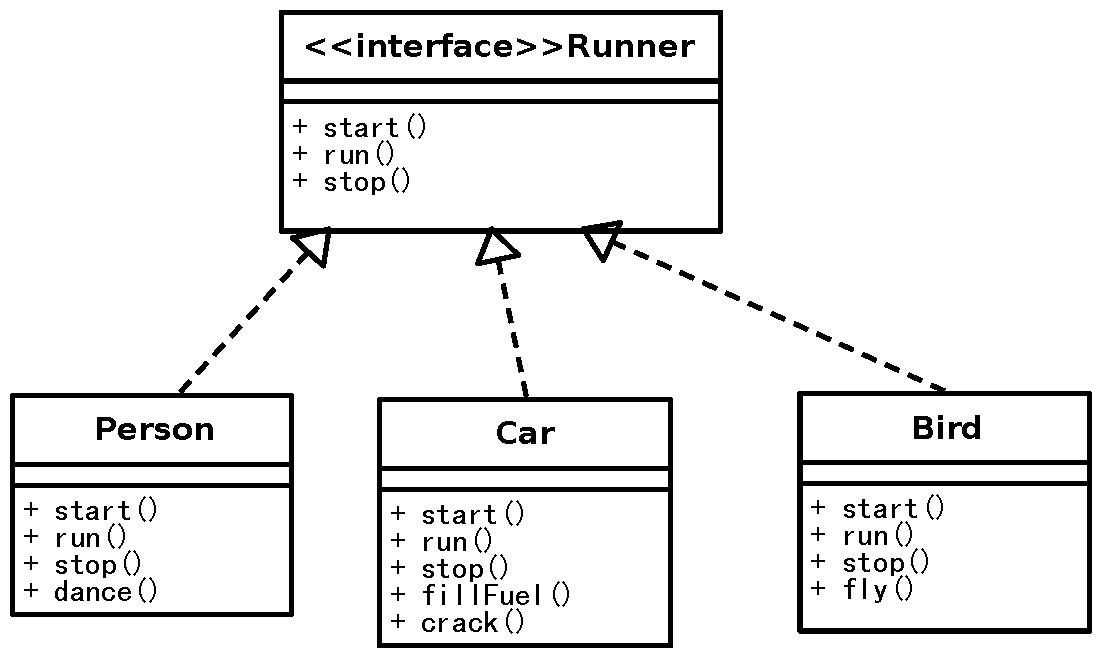
\includegraphics[width=0.5\textwidth]{a.pdf}
  \end{figure}

  \notice{类允许实现多重接口}

  \codeset{package sample.advance.interfacesample}

\end{frame}


\begin{frame}[fragile] % [fragile]参数使得能够插入代码
\frametitle{接口间的继承}

与接口的多重实现情况类似,由于不担心方法追溯调用上的不确定性,接口之间
的继承允许“多重继承”的情况。

\begin{javaCode}
interface A {
  public void ma();
}
interface B {
  public int mb(int i);
}
interface C extends A,B {  //接口的多重继承
  public String mc();
}
class D implements C {
  public void ma() {
    System.out.println("Implements method ma()!");
  }
  public int mb(int i) {
    return 2000 + i;
  }
  public String mc() {
    return "Hello!";
  }
}
\end{javaCode}
{\footnotesize \Mage 上述代码中的D类缺省继承了Object类,直接实现了接口C,间接实现了接口A和B,由于多态性的机
制,将来D类的对象可以当作Object、C、A或B等类型使用。}
\end{frame}

\begin{frame}[fragile] % [fragile]参数使得能够插入代码
  \frametitle{接口特性总结}

  \begin{itemize}[<+-| alert@+>]
  \item 通过接口可以实现不相关类的相同行为,而不需要考虑这些类之间的层次关系。
  \item 接口可以被多重实现。
  \item 接口可以继承其它的接口,并添加新的属性和抽象方法,接口间支持多重继承。
  \end{itemize}
\end{frame}
%%%%%%%%%%%%%%%%%%%%%%%%%%%%%%%%%%%%%%%%%%%%%%%%
\section{抽象类和接口剖析}

\begin{frame}[fragile]
  \frametitle{语法层面的区别}

  \begin{alertblock}{}
    \hei\centering 概念差异 —— 语法差异 —— 用法差异 —— 设计哲学
  \end{alertblock}

  \pause
  
  \begin{itemize}[<+-| alert@+>]
  \item 抽象类可以提供成员方法的实现细节,而接口中只能存在public
    abstract方法
  \item 抽象类中的成员变量可以为各种类型,而接口中的成员变量只能
    是public static final类型
  \item 抽象类可以有静态代码块和静态方法,接口中不能含有静态代码块以及
    静态方法
  \item 一个类只能继承一个抽象类,而一个类却可以实现多个接口
  \end{itemize}
\end{frame}

\begin{frame}[fragile]
  \frametitle{设计层面的区别}

  \begin{block}{}
    \begin{itemize}\kai
    \item 抽象类是对类的抽象(可以抽象但不宜实例化),而接口是对行为的
      抽象。
    \item 抽象类是对类整体进行抽象,包括属性、行为,但是接口却是对类局
      部(行为)进行抽象。
    \end{itemize}
  \end{block}

  \pause

  \begin{block}{}
    \begin{itemize}\kai
    \item 抽象类作为很多子类的父类,它是一种模板式设计。{\Red 模板式设计:模
      板代表公共部分,公共部分需要改的则改动模板即可。}
    \item 而接口是一种行为规范,它是一种辐射式设计。{\Red 辐射式设计:接口
      进行了变更,则所有实现类都必须进行相应的改动。}
    \end{itemize}
  \end{block}  

\end{frame}

\begin{frame}[fragile]
  \frametitle{怎样才是合理的设计?(门和警报的示例)}

  一般来说,门都有\fbox{open()}和\fbox{close()}这两个动作。通过抽象类和
  接口来定义这个抽象概念:

  \begin{columns}
    \column{0.5\textwidth}

    \begin{javaCode}
      abstract class Door {
        public abstract void open();
        public abstract void close();
      }
    \end{javaCode}
    \column{0.5\textwidth}

    \begin{javaCode}
      interface Door {
        public abstract void open();
        public abstract void close();
      }
    \end{javaCode}
  \end{columns}

  \pause
  
  \notice{问题} 如果现在我们需要门具有报警\fbox{alarm()}的功能该如何实
  现?
\end{frame}

\begin{frame}[fragile]
  \frametitle{怎样才是合理的设计?(门和警报的示例)}

  \tta{思路一} 
  
  将这三个功能都放在抽象类里面,这样一来所有继承这个抽象类的子类都具备
  了报警功能,但是有的门并不一定需要具备报警功能。\pause {\hei\Red 不合理抽象}

  \pause
  
  \tta{思路二} 

  将这三个功能都放在接口里面,但需要用到报警功能的类就需要实现这个接口
  中的open()和close(),也许这个类根本就不具备open()和close()这两个功能,
  比如火灾报警器。\pause {\hei\Red 不合理规划}

\end{frame}

\begin{frame}[fragile]
  \frametitle{怎样才是合理的设计?(门和警报的示例)}

  Door的open() 、close()和alarm()根本就属于两个不同范畴内的行为:

  \begin{itemize}
  \item open()和close()属于门本身固有的行为特性。
  \item alarm()属于延伸的附加行为。
  \end{itemize}

  \pause
  
  \tta{更为合理的思路} 

  \ding{182} 单独将报警设计为一个接口,包含alarm()行为;\ding{183} Door设计为单独
  的抽象类,包含open()和close()两种行为;\ding{184} 设计一个报警门继
  承Door类和实现Alarm接口。

  \codeset{package sample.advance.door}
\end{frame}



%% 1)抽象类是对一种事物的抽象,即对类抽象,而接口是对行为的抽象。抽象类是对整个类整体进行抽象,包括属性、行为,但是接口却是对类局部(行为)进行抽象。举个简单的例子,飞机和鸟是不同类的事物,但是它们都有一个共性,就是都会飞。那么在设计的时候,可以将飞机设计为一个类Airplane,将鸟设计为一个类Bird,但是不能将 飞行 这个特性也设计为类,因此它只是一个行为特性,并不是对一类事物的抽象描述。此时可以将 飞行 设计为一个接口Fly,包含方法fly(),然后Airplane和Bird分别根据自己的需要实现Fly这个接口。然后至于有不同种类的飞机,比如战斗机、民用飞机等直接继承Airplane即可,对于鸟也是类似的,不同种类的鸟直接继承Bird类即可。从这里可以看出,继承是一个 "是不是"的关系,而 接口 实现则是 "有没有"的关系。如果一个类继承了某个抽象类,则子类必定是抽象类的种类,而接口实现则是有没有、具备不具备的关系,比如鸟是否能飞(或者是否具备飞行这个特点),能飞行则可以实现这个接口,不能飞行就不实现这个接口。
%%
%% 2)设计层面不同,抽象类作为很多子类的父类,它是一种模板式设计。而接口是一种行为规范,它是一种辐射式设计。什么是模板式设计?最简单例子,大家都用过ppt里面的模板,如果用模板A设计了ppt B和ppt C,ppt B和ppt C公共的部分就是模板A了,如果它们的公共部分需要改动,则只需要改动模板A就可以了,不需要重新对ppt B和ppt C进行改动。而辐射式设计,比如某个电梯都装了某种报警器,一旦要更新报警器,就必须全部更新。也就是说对于抽象类,如果需要添加新的方法,可以直接在抽象类中添加具体的实现,子类可以不进行变更;而对于接口则不行,如果接口进行了变更,则所有实现这个接口的类都必须进行相应的改动。
%%
%% 下面看一个网上流传最广泛的例子:门和警报的例子:门都有open( )和close( )两个动作,此时我们可以定义通过抽象类和接口来定义这个抽象概念:
%%
%%
%%abstract class Door {
%%    public abstract void open();
%%    public abstract void close();
%%}
%%  或者:
%%
%%interface Door {
%%    public abstract void open();
%%    public abstract void close();
%%}
%%  但是现在如果我们需要门具有报警alarm( )的功能,那么该如何实现?下面提供两种思路:
%%


%%%%%%%%%%%%%%%%%%%%%%%%%%%%%%%%%%%%%%%%%%%%%%%%
\section{嵌套类}
\begin{frame}[fragile] % [fragile]参数使得能够插入代码
  \frametitle{什么是嵌套类}

  Java语言支持类的嵌套定义,即允许将一个类定义在其他类的内部,其中内层的类被称为嵌套类。

  \tta{嵌套类的分类}
  
  \begin{description}
  \item[\fbox{静态嵌套类(Static Nested Class)}] 使用static修饰的嵌套类
  \item[\fbox{内部类(Inner Class)}] 非static的嵌套类
    \begin{description}
    \item[普通内部类] 在类中的方法或语句块外部定义的非static类。
    \item[局部内部类] 定义在方法或语句块中的类,也称局部类。
    \item[匿名内部类] 定义在方法或语句块中,该类没有名字、只能在其所在
      之处使用一次。
    \end{description}
  \end{description}

  {\kai (仅讲授包含静态嵌套类和匿名内部类,其他自行学习)}
  
\end{frame}


\begin{frame}[fragile] % [fragile]参数使得能够插入代码
  \frametitle{静态嵌套类}

  \tta{静态嵌套类的特征}
  
  \begin{itemize}
  \item {\hei 静态嵌套类不再依赖/引用外层类的特定对象,只是隐藏在另一个
      类中而已。}
  \item 由于静态嵌套类的对象不依赖外层类的对象而独立存在,因而可以直接
    创建,进而也就无法在静态嵌套类中直接使用其外层类的非static成员。
  \end{itemize}

  \codeset{sample.advance.nestedclass.StaticNestedClassSample.java}
\end{frame}

%%\begin{frame}[fragile] % [fragile]参数使得能够插入代码
%%\frametitle{使用内部类\ding{182}}
%%
%%\samp{JavaSE\_03/TestInnerClass.java}
%%
%%\samp{TestInner.java}
%%\begin{javaCode}
%%class A {
%%  private int s;
%%  public class B {
%%    public void mb() {
%%      s = 100;
%%      System.out.println("在内部类 B 中 s=" + s);
%%    }
%%  }
%%  public void ma() {
%%    B i = new B();
%%    i.mb();
%%  }
%%}
%%
%%public class TestInner {
%%  public static void main(String args[]) {
%%    A o = new A();
%%    o.ma();
%%  }
%%}
%%\end{javaCode}
%%
%%{\small \Mage 上述程序编译后生成三个文件:TestInner.class, A.class, A\$B.class。}
%%\end{frame}
%%
%%\begin{frame}[fragile] % [fragile]参数使得能够插入代码
%%\frametitle{使用内部类\ding{182}}
%%
%%\wxd{TestInner.java运行时的内存状态}
%%
%%系统创建一个外层类的对象o,并将其实例变量s缺省初始化为0。
%%
%%\begin{figure}
%%\centering
%%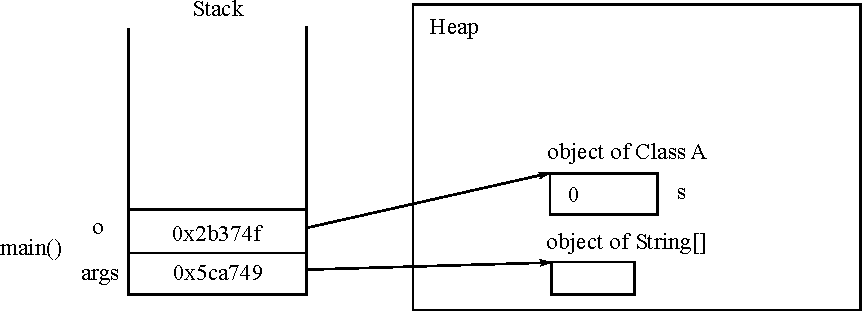
\includegraphics[width=0.8\textwidth]{innerclass01.pdf}
%%\end{figure}
%%
%%\end{frame}
%%
%%\begin{frame}[fragile] % [fragile]参数使得能够插入代码
%%\frametitle{使用内部类\ding{182}}
%%
%%\wxd{TestInner.java运行时的内存状态}
%%
%%调用对象o的成员方法ma(),首先为引用变量this分配空间以记录该方法本次运行时的当前对象,然后执行方法体中的第一条语句创建一个内部类B的对象i。
%%
%%\begin{figure}
%%\centering
%%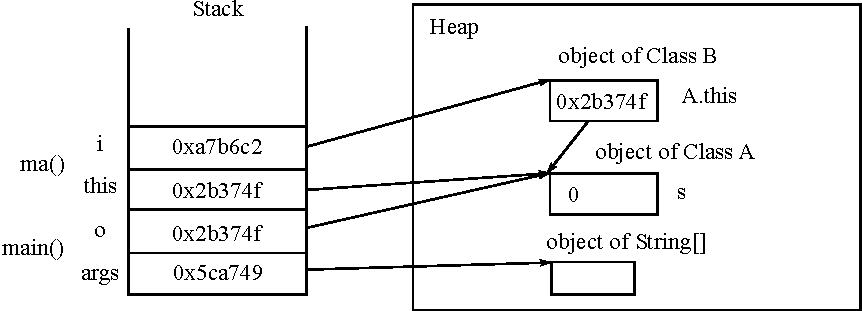
\includegraphics[width=0.8\textwidth]{innerclass02.pdf}
%%\end{figure}
%%
%%{\kai\small 此时,内部类B中虽然未显式的定义任何属性,但其对象i一经创建,即拥有一个系统自动添加的属性(实例变量),该属性的数据类型为外层类对象的句柄,该属性为只读,且可以使用约定标记<外层类名>.this访问。}
%%
%%\end{frame}
%%
%%\begin{frame}[fragile] % [fragile]参数使得能够插入代码
%%\frametitle{使用内部类\ding{182}}
%%
%%\wxd{TestInner.java运行时的内存状态}
%%
%%内部类对象i调用其成员方法mb()。
%%
%%\begin{figure}
%%\centering
%%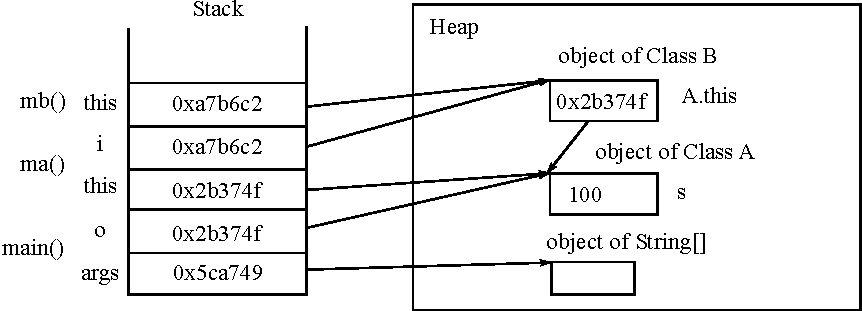
\includegraphics[width=0.8\textwidth]{innerclass03.pdf}
%%\end{figure}
%%
%%{\kai\small 在方法体中遇到变量s时,按照如下处理过程:首先在当前方法mb()中检索是否存在局部变量(包括方法形参)s,没有则继续查找方法的当前对象(内部类B中)是否存在成员变量s,没有则通过属性A.this检索当前对象所依赖的外层类对象,最终找到并操作该变量s并赋值为100。}
%%\end{frame}
%%
%%\begin{frame}[fragile] % [fragile]参数使得能够插入代码
%%\frametitle{使用内部类\ding{183}}
%%
%%在外部使用其他类中的内部类虽然不提倡,但也是允许的。此时,应指明其完整层次,并显式建立对
%%象间的依赖关系。
%%
%%\samp{A.java}
%%\begin{javaCode}
%%public class A {
%%  private int s;
%%  public class B {
%%    public void mb() {
%%      System.out.println(s);
%%    }
%%  }
%%}
%%\end{javaCode}
%%\samp{TestInner2.java}
%%\begin{javaCode}
%%public class TestInner2 {
%%  public static void main(String[] args) {
%%    A a = new A();
%%    // 创建一个依赖于 a 而存在的 b
%%    A.B b = a.new B();
%%    b.mb();
%%  }
%%}
%%\end{javaCode}
%%\end{frame}
%%
%%\begin{frame}[fragile] % [fragile]参数使得能够插入代码
%%\frametitle{使用内部类\ding{184}}
%%
%%内部类中出现变量命名冲突时,可以使用内部类对象的特殊属性“<外层类名>.this”来访问其所依赖
%%外层类对象的成员。
%%\samp{TestInner3.class}
%%\begin{javaCode}
%%class A {
%%  private int s = 111;
%%  public class B {
%%    private int s = 222;
%%    public void mb(int s) {
%%      System.out.println(s);  // 局部变量 s
%%      System.out.println(this.s);  // 内部类对象的属性 s
%%      System.out.println(A.this.s); // 外层类对象属性 s
%%    }
%%  }
%%}
%%
%%public class TestInner3 {
%%  public static void main(String args[]) {
%%    A a = new A();
%%    A.B b = a.new B();
%%    b.mb(333);
%%  }
%%}
%%\end{javaCode}
%%{\small\Mage 输出结果为:333\textbackslash n 222\textbackslash n 111}
%%\end{frame}
%%
%%\begin{frame}[fragile] % [fragile]参数使得能够插入代码
%%\frametitle{局部内部类}
%%
%%局部内部类是定义在Java方法或语句块中的类型,相当于方法中的局部变量,其作用域仅限于其所在的方法体或者语句块。
%%
%%\begin{itemize}\kai
%%\item 局部类声明时不允许加public、private等访问控制修饰符。
%%\item 局部类也不允许定义static属性和方法,{\Red 除非局部类为静态类(后续讲述)}。
%%\item 局部类中不但可以访问其所在外层类的成员,还可以访问其所在方法/语句块中的局部变量,但
%%  这些变量必须声明为{\Red final}。
%%\end{itemize}
%%
%%\samp{JavaSE\_03/TestLocalInnerClass.java}
%%
%%{\hei\Red 不建议使用局部类。}
%%\end{frame}

\begin{frame}[fragile] % [fragile]参数使得能够插入代码
\frametitle{匿名内部类}

匿名内部类是局部类的一种简化。

{\kai 当我们只在一处使用到某个类型时,可以将之定义为局部类,进而如果我
  们只是创建并使用该类的一个实例的话,那么连类的名字都可以省略。}
\end{frame}

\begin{frame}[fragile] % [fragile]参数使得能够插入代码
  \frametitle{使用匿名内部类}

  \samp{Person.java}

  \begin{javaCode}
    public abstract class Person {
      private String name;
      private int age;
      
      public Person() {}
      
      public Person(String name, int age) {
        this.name = name;
        this.age = age;
      }
      
      public String getInfo() {
        return "Name: " + name + "\t Age: " + age;
      }
      
      public abstract void work();
    }  
  \end{javaCode}
\end{frame}

\begin{frame}[fragile] % [fragile]参数使得能够插入代码
  \frametitle{使用匿名内部类}

  \samp{TestAnonymous.java}

  \begin{javaCode}
    public class TestAnonymous {
      public static void main(String[] args) {
        Person sp = new Person() { \\ 匿名内部类
          public void work() {
            System.out.println("个人信息:" + this.getInfo());
            System.out.println("I am sailing.");
          }
        };
        
        sp.work();
      }
    }
  \end{javaCode}

  \pause
  
  \ttc{上述代码的解释}

  {\small\Red 定义一个新的Java内部类,该类本身没有名字,但继承了指定的父
    类Person,并在此匿名子类中重写了父类的work()方法,然后立即创建了一
    个该匿名子类的对象,再将其地址保存到引用变量sp中待用。}
\end{frame}

\begin{frame}[fragile] % [fragile]参数使得能够插入代码
  \frametitle{使用匿名内部类}

  由于匿名类没有类名,而构造方法必须与类同名,所以{\hei 匿名类不能显式的定义构造方
    法},但系统允许在创建匿名类对象时将参数传给父类构造方法(使用父类的构造方法)。

  \begin{javaCode}
    Person sp = new Person("Kevin", 30) {
      public void work() {
        System.out.println("个人信息:" + this.getInfo());
        System.out.println("I am sailing.");
      }
    };
  \end{javaCode}
\end{frame}

\begin{frame}[fragile] % [fragile]参数使得能够插入代码
  \frametitle{使用匿名内部类}

  匿名类除了可以继承现有父类之外,还可以实现接口,但不允许实现多个接口,
  且实现接口时就不能再继承父类了,反之亦然。

  \samp{Swimmer.java}

  \begin{javaCode}
    public interface Swimmer {
      public abstract void swim();
    }
  \end{javaCode}

  \samp{TestAnonymous2.java}
  
  \begin{javaCode}
    public class TestAnonymous2 {
      public static void main(String[] args) {
        TestAnonymous2 ta = new TestAnonymous2();
        ta.test(new Swimmer() { // 匿名类实现接口
          public void swim() {
            System.out.println("I am swimming.");
          }
        });
        
        public void test(Swimmer swimmer) {
          swimmer.swim();
        }
      }
    \end{javaCode}
\end{frame}

\section{枚举类型}

\begin{frame}[fragile] % [fragile]参数使得能够插入代码
  \frametitle{枚举类型}

  \begin{block}{}
    Java SE 5.0开始,引入了一种新的引用数据结构{\hei\Red 枚举类
      型}。{\kai 枚举类型均自动继承java.lang.Enum类,使用一组常量值来表示
      特定的数据集合,该集合中数据的数目确定(通常较少),且这些数据只能
      取预先定义的值。}
  \end{block}

  \pause
  \begin{javaCode}
    public enum Week {
      MON, TUE, WED, THU, FRI, SAT, SUN
    }
  \end{javaCode}
  \pause
  \notice{无枚举类型前如何解决上述需求?}

  一般采用声明多个整型常量的做法实现枚举类的功能。

  \begin{javaCode}
    public class Week {
      public static final int MON = 1;
      public static final int TUE = 2;
      ...
    }    
  \end{javaCode}
\end{frame}

%%\begin{frame}[fragile] % [fragile]参数使得能够插入代码
%%\frametitle{使用枚举类型}
%%\begin{javaCode}
%%public enum Week {
%%  MON, TUE, WED, THU, FRI, SAT, SUN
%%}  
%%\end{javaCode}
%%\begin{javaCode}
%%public class TestEnum {
%%  public static void main(String[] args) {
%%    TestEnum te = new TestEnum();
%%    te.work(Week.SUN);
%%  }
%%  public void work(Week day) {
%%    if (day.equals(Week.SAT)) {
%%      System.out.println("购物!");
%%    }else if (day.equals(Week.SUN)) {
%%      System.out.println("祈祷!");
%%    } else {
%%      System.out.println("工作!");
%%    }
%%  }
%%}
%%\end{javaCode}
%%\end{frame}

%%\begin{frame}[fragile] % [fragile]参数使得能够插入代码
%%\frametitle{遍历枚举类型常量值}
%%
%%可以使用静态方法values()遍历枚举类型常量值。
%%
%%\samp{ListEnum.java}
%%\begin{javaCode}
%%public class ListEnum {
%%  public static void main(String[] args) {
%%    Week[] days = Week.values();
%%    for(Week d: days) {
%%      System.out.println(d);
%%    }
%%  }
%%}
%%\end{javaCode}
%%\end{frame}

\begin{frame}[fragile] % [fragile]参数使得能够插入代码
\frametitle{组合使用枚举类型与switch}

\codeset{package sample.advance.enumclass}

\pause

\notice{注意}

\begin{enumerate}
\item case字句必须省略其枚举类型的前缀,即只需要写成 case SUN:,而不允许写成 case
  Week.SUN:,否则编译出错。
\item 不必担心系统无法搞清这些常量名称的出处,因为switch后的小括号中的表达式已经指明本次
  要区分处理的是Week类型常量。
\end{enumerate}
\end{frame}

\begin{frame}[fragile]
  \frametitle{本节习题}

  \wxd{简答题}
  \begin{enumerate}
  \item 分析抽象类和接口的异同,说明抽象类和接口的作用。
  \end{enumerate}

  \wxd{小编程}
  \begin{enumerate}
  \item 为Eclipse安装Amateras插件
    (https://takezoe.github.io/amateras-update-site/),并尝试使用该插
    件为示例代码或自己编写的代码自动生成类图。
  \end{enumerate}

\end{frame}



% TKS %%%%%%%%%%%%%%%%%%%%%%%%%%%%%%%%%%%%%%%%%%%%%%
\begin{frame}[focus]
\centering
{\Huge {THE END}} \\
\vspace{5mm}
{\Large wangxiaodong@ouc.edu.cn} \\
\end{frame}
%%%%%%%%%%%%%%%%%%%%%%%%%%%%%%%%%%%%%%%%%%%%%%%%%%%%
\end{document}
